\section{Internet}

\begin{definition}[\textit{Internet}]
    The Internet is a global network that connects various types of networks, enabling communication and data exchange.
\end{definition}
Traditionally, the internet was primarily used for fixed, stationary clients accessing well-defined services. 
However, modern internet usage has shifted significantly with the rise of mobile clients. 
These mobile devices, often equipped with sensing and actuating capabilities, are no longer just consumers of information and services.

\paragraph*{Technological advancements}
Several breakthroughs have paved the way for the rapid growth of the Internet of Things. 
The miniaturization of hardware has enabled the development of compact yet powerful smart devices. 
At the same time, improvements in energy solutions have enhanced the efficiency and autonomy of these devices. 
Increased mobility has further expanded the reach and functionality of Internet of Things applications.

In parallel, communication protocols have evolved to support low-power wireless technologies, ensuring efficient and reliable connectivity. 
The widespread adoption of cloud computing has also played a crucial role, providing scalable architectures and vast processing power. 
Additionally, the rise of Artificial Intelligence has unlocked new possibilities for intelligent data analysis, automation, and decision-making within Internet of Things ecosystems.

\subsection{Internet of Things}
\begin{definition}[\textit{Internet of Things}]
    The Internet of Things is a worldwide network of uniquely addressable interconnected objects, based on standard communication.
\end{definition}
\noindent The Internet of Things is based on: 
\begin{itemize}
    \item \textit{Smart objects}: devices embedded with sensors, actuators, and connectivity.
    \item \textit{Data}: continuous collection and processing of information.
    \item \textit{Pervasiveness}: seamless integration into everyday life.
    \item \textit{Seamless communication}: reliable and efficient interaction between devices, networks, and services.
\end{itemize}
\noindent The Internet of Things primarily consists of connected low-cost endpoints, such as consumer devices and everyday smart objects, which focus on accessibility and widespread adoption.

\subsection{Industrial Internet of Things}
\begin{definition}[\textit{Industrial Internet of Things}]
    The Industrial Internet of Things refers to a network of interconnected sensors, instruments, and devices integrated with industrial computing applications, including manufacturing, energy management, and automation.
\end{definition}
The Industrial Internet of Things consists of connected industrial assets that are typically medium to high-cost. 
These devices are more expensive but also more responsive.

Cybersecurity is a central concern in the Industrial Internet of Things, where even minor disruptions can have severe consequences. 
Unlike consumer Internet of Things, Industrial Internet of Things systems must operate with continuous availability, robustness, and resiliency, ensuring that industrial processes remain uninterrupted.
Industrial Internet of Things environments often coexist with a significant amount of legacy operational technologies. 
These legacy systems, designed for reliability rather than cybersecurity, introduce additional challenges in securing industrial networks.

While usability and user experience are critical in consumer Internet of Things, they are not primary concerns in Industrial Internet of Things. 
Instead, the focus is on system integrity, fault tolerance, and maintaining operational continuity in complex industrial ecosystems.

\subsection{Architecture}
The Internet of Things endpoints require strong security and reliability. 
These devices are not just about connectivity; they depend on a combination of smart objects, reliable connectivity, data collection, and advanced analytics to function properly.
The security of Internet of Things endpoints is critical. 
Ensuring reliability ensures that these devices can perform their tasks without interruption.
\begin{figure}[H]
    \centering
    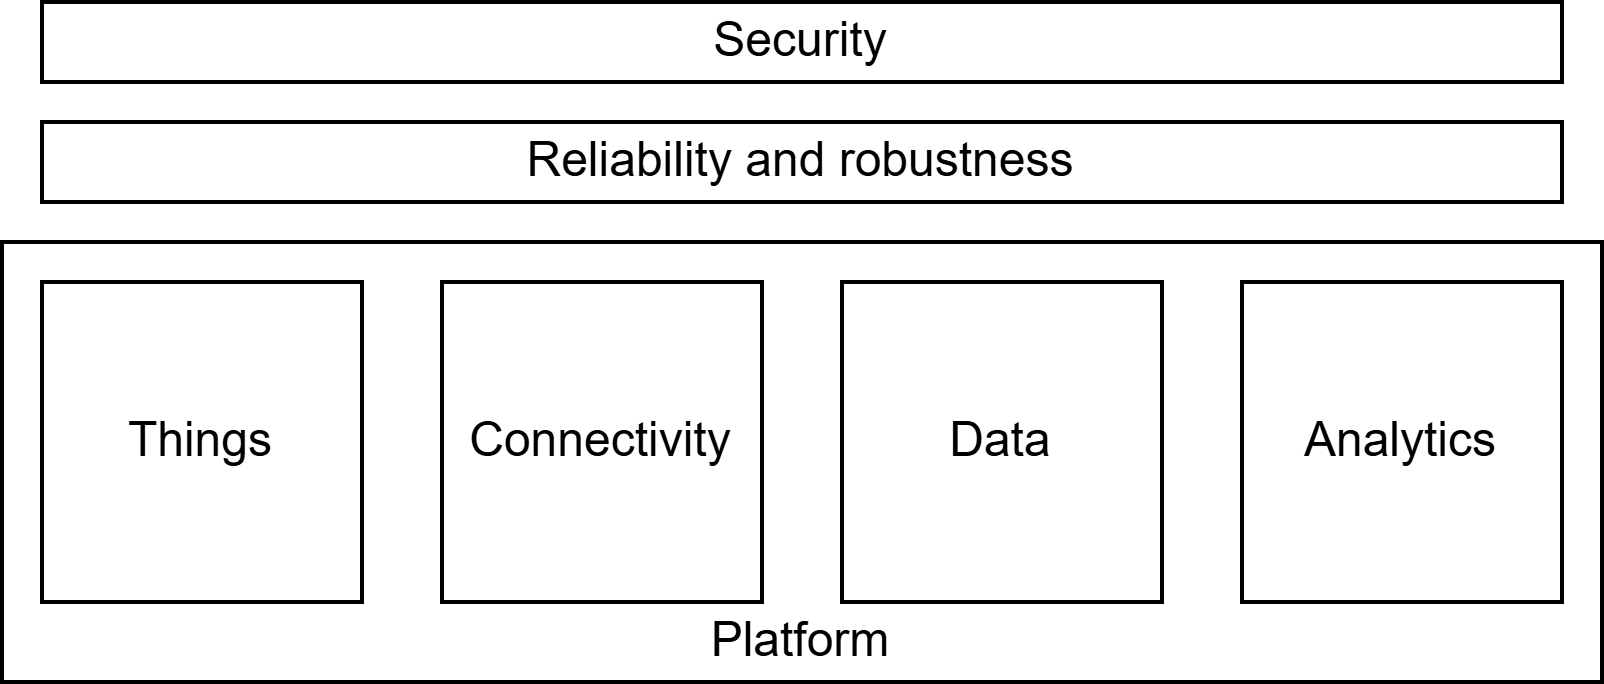
\includegraphics[width=0.75\linewidth]{images/iot1.png}
    \caption{Internet of Things architecture}
\end{figure}